\documentclass[../poliXuniversity_hospital_(USP)_report.tex]{subfiles}

\begin{document}
\chapter{Software ciclo}

\section{Algorítimo de movimentação}

\subsection{Máquina de estados}
Seguindo o mesmo raciocinio do Golgi bot, foi usado maquina de estados para definir e controlar o comportamento da maquina. Foram estabelecidos os seguinte estados:

MODE: Durante esse estado é solicidado via LCD o modo de operação da máquina, Manual, no qual o profissional da saude escolhe entre atividade ativa livre, ativa resistida ou passiva. Já o automático, o ESP32 coleta dados de velocidade e torque para definir qual é o modo de operação mais adequado para aquele paciente. Após a seleção do modo o estado é alterado para TIMER
  
TIMER: Neste modo é solicidado via LCD a duração desejada do exercicio, de 0 a 30 minutos. Após a seleção da duração o estado é alterado para SET VEL
 
SET VEL: Para o modo de opera~~ao passivo, no qual o motor auxilia o movimento, é uma parâmetro importante para a fisioterapia a velocidade em RPM que deve ser mantiada constante, para isso é solicidado ao fisioterapeuta a velocidade alvo desejada. Apos a definição o estado é alterado para SET DRAG.
 
SET DRAG: Assim como o RPM a resistencia(kg*m) oferecida no modo ativo resistido, no qual o motor oferece resistência ao movimento, é um parametro importante para mensurar a evolução do tratamento. Por isso é solicidado via LCD a resistencia de 1,2 ou 3 Kg*m. Após a configuração o exercicio é iniciao e o estado ira ser definido pela função check state que no modo manual escolhe o estado(STAND BY, ACTIVE PLUS, PASSIVE ou DONE, caso o exercicio acabe) fornecido pelo potenciomentro seletor e no modo Automático é definido pelo algoritimo de diagnosticação automático.
 
STAND BY : Nesse modo o paciente realiza a pedalada livre, sem influência do motor.
 
 ACTIVE PLUS: O exercício agora é influênciado pelo motor, o qual resiste o movimento, o torque fornecido é estimado constante devido ao algoritimo de controle do motor que usa como realimentação o sinal do sensor de corrente.
 
 FADE: Modo criado para transição entre o STAND BY e o PASSIVE, para evitar arrancada brusca do motor e adicionar conforto no exercicio o motor é ativado gradualmente.
 
 PASSIVE: Agora o exercicio é totalmente auxiliado pelo motor, o qual mantem o RPM constante usando o algoritimo de controle realimento pela velocidade lida pelo Encoder.
 
 DONE: Com o fim da duração do exercicio o estado DONE é ativado e nele todo movimento é encerrado e no display LCD é mostrado o relatorio de exercicio, quatidade de rotações feitas em cada modo. Caso qualquer botão seja apertado, a máquina reinicia e pode ser reconfigurada, o estado é alterado para RESET.
 
 RESET: O microcontrolador é reiniciado e o estado é alterado para MODE.

\subsection{Controle PID}
Com a mesma bibiblioteca desenvolvida para o controle do Golgi-bot foi implementado o dois controladores para o Ciclo Ergômetro. Um para o modo passivo, no qual o intuito é manter a velocidade(RPM) constante e igual a velocidade alvo. Já o segundo atua no modo Ativo resistido que tenta mandar o torque constante e igual ao arrasto alvo setado ao inciar a máquina. 


\begin{figure}[h]
\centering
     \caption{Diagrama de blocos Controle RPM}
        \centering % para centralizarmos a figura
        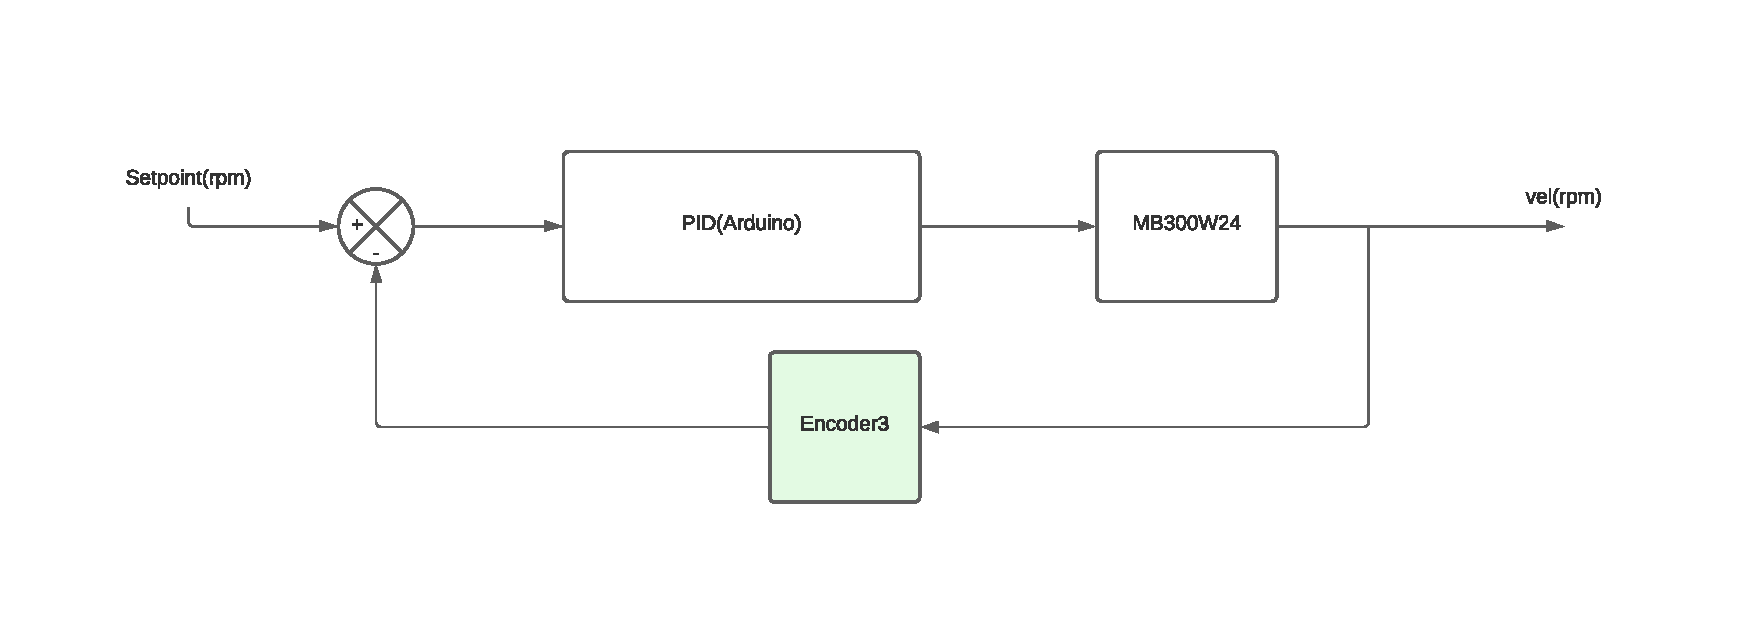
\includegraphics[width=10cm]{images/Diagrama de blocos RPM.pdf}
        \caption*{Fonte: Autor}
        \label{figura: Diagrama de blocos Controle RPM}
\end{figure}

\begin{figure}[h]
\centering
    \caption{Diagrama de blocos Controle Torque}
        \centering % para centralizarmos a figura
        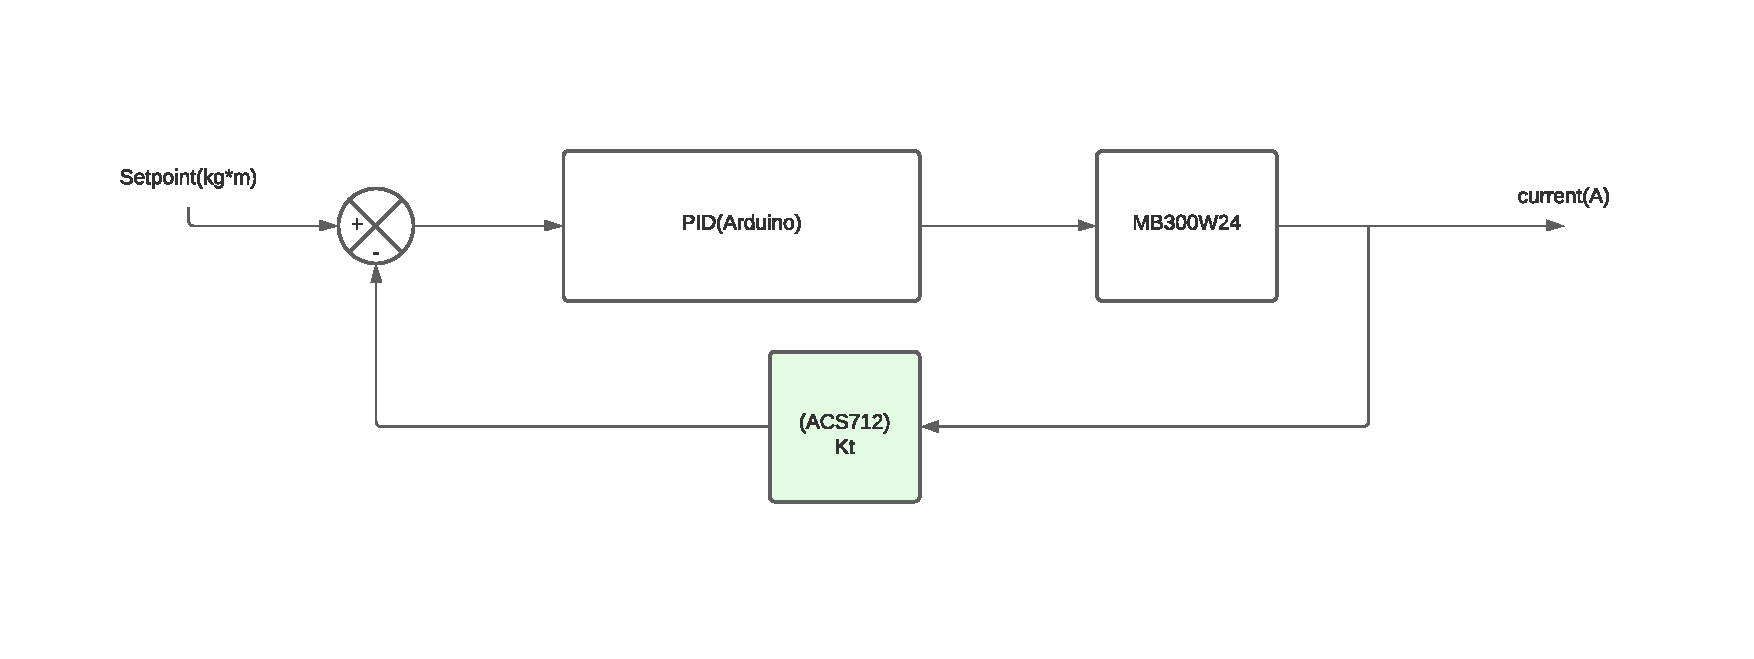
\includegraphics[width=10cm]{images/Diagrama de blocos Torque.pdf}
        \caption*{Fonte: Autor}
        \label{figura: Diagrama de blocos Controle em Z}
\end{figure}

\section{Interface com usuários}

\subsection{Configuração de exercicio}
Para que seja usado de maneira a melhorar a saúde do paciente, é essencial que o estado de saúde do paciente seja analisado pelo fisioterapeuta e com a sua conclusão é possivel ajustar parâmetros como duração do exercício, velocidade em RPM e resistência. Para isso foi implementado um visor LCD no qual é solicidado todas essas informações antes de iniciar o exercício. Com essas parametrizações é possível analisar 

\subsection{Coleta e amostra de parâmetros}

A fim de auxiliar a melhoria da qualidade do serviço de fisioterapia foi implementado a coleta de parametros que mensuram a saúde e evolução do paciente. Os parametros coletados são, velocidade média, esforço médio, número de ciclos realizado em cada modo de operação e tempo de exercicio. Todo sistema de aquisição de dados foi representado em tópicos anteriores, os quais ja eram usados no controle de velocidade e resistência, foi adicionado apenas a funcionalidade de armazenamento.

\end{document}